
		\section{Standard Antichess}
	
		Antichess is a variant of chess in which the goal is to either lose all of 
		your pieces (except your king) or checkmate your opponent.
		
		\subsection{The Chessboard}
		
		Antichess is played between two opponents by moving pieces on a square board. 
		The board is composed of 64 equal squares. The eight vertical lines of squares 
		are called columns. The eight horizontal lines of squares are called rows. The 
		squares are colored black and white alternately. The lines of squares of the 
		same color, touching corner to corner, are called diagonals. The chessboard is 
		placed between the players in such a way that the near corner to the right of 
		each player is white. The columns are labeled a to h from left to right. The 
		rows are numbered 1 to 8 from bottom to top.
		
		\subsection{The Pieces}
		
		At the beginning of the game, one player ("white") has 16 white pieces, and the 
		other ("black") has 16 black pieces. The white player pieces are: one King (e1), 
		one Queen (d1), two bishops (c1 and f1), two knights (b1 and g1), two rooks 
		(a1 and h1), and eight pawns (row 2). The black player pieces are: one King 
		(e8), one Queen (d8), two bishops (c8 and f8), two knights (b8 and g8), two rooks 
		(a8 and h8), and eight pawns (row 7). The initial position of the pieces on the 
		chessboard is shown in Figure ().
		
		%%% Initial Position of pieces
				\begin{figure}
					\begin{center}
						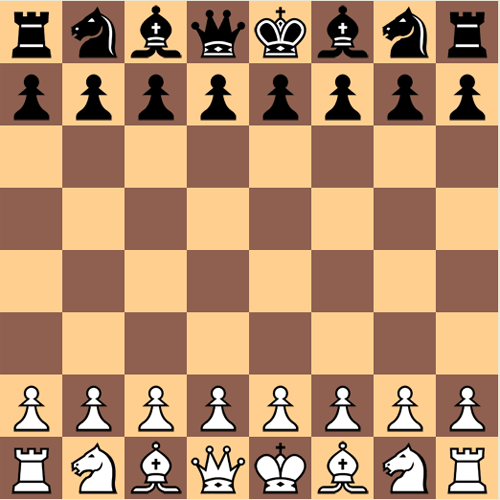
\includegraphics[width=200pt]{img/initial-position.png}
							\caption{Initial position of the pieces}						
					\end{center}
				\end{figure}
				
		\subsection{The moves}
		
		A move is defined by the following rules:
		
			\begin{enumerate}
				\item White moves first. The players alternate in making one move at a time
				 			until the game is completed.
				\item A move is the transfer by a player of one of his pieces from one 
							square to another square, which is either vacant or occupied by an 
							opponent's piece.
				\item No piece except the knight may cross a square occupied by another 
							piece. That is, only the knight may jump over other pieces.
				\item A piece played to a square occupied by an opponent's piece captures 
							that piece as part of the same move. The captured piece is immediately 
							removed from the board.
			\end{enumerate}
			
		A player's moves are limited by the following fact: A player is forced to capture 
		an opponent's piece whenever possible. If a player can take several of the 
		opponent's pieces, he/she is free to choose which piece to take. This limitation 
		does not exists in regular chess. The only exception to this rule is being in check.

		All the pieces move exactly as they do in standard chess. An excellent description 
		of how each piece moves and captures is at 
			\begin{center}
				\url{http://www.princeton.edu/~jedwards/cif/chess.html} 
			\end{center}
		
		In the Standard Antichess rules:
			\begin{itemize}
				\item Castling and en passant are \textbf{not} allowed.
				\item When a pawn moves to the last row on the opposing side, it turns into a 
							queen. (In standard chess, such a pawn can be turned into any piece of 
							the player's choice.)
			\end{itemize}
			
		\subsection{Handling Check Situations}
		
		In short, each move of player A must observe the following:
			\begin{enumerate}
				\item If A's king is under check, A must move the king out of check.
				\item A cannot move in a way that causes the king to come into check.
				\item If A can take one of B's pieces, then it must (unless disallowed by 
							the previous rule).
				\item If A's king is under check and A can move in such a way that the king 
							is out of check by either taking B's piece or in some other manner, A 
							must take B's piece.
			\end{enumerate}

		The king is in check when the square it occupies is attackable by one or more 
		of the opponent's pieces; in this case, the latter is/are said to be checking 
		the king. A player may not make a move which leaves his king on a square 
		attackable by any of his opponent's pieces; e.g., the player cannot move the 
		king into check. Check must be resolved by the move immediately following. If 
		any check cannot be parried, the king is said to be checkmated or mated.

		It is the foremost obligation of each player to move the king out of a check. 
		This overrides the rule that you must take an opponent's piece. For example, 
		in the figure below to the left, it is black's turn and black must move its 
		king out of check even though it can take white's bishop on c6 with its rook.

		If it is possible for a player to remove the king from check as well take a 
		piece of the opponent, then the player must do so. For example, suppose the 
		black player's king is under check from white's rook. Further, suppose black 
		has two choices to move away from check � remove the check with or without 
		taking a white piece. In that case, black must take white's piece and remove 
		the check. In the figure below to the right, black's king must take the white 
		bishop with the king in the next move (it cannot simply move the king away 
		from check without taking the bishop).	
		
		\subsection{End of Game}
		
		Player A wins the game against player B if:
			\begin{enumerate}
				\item all pieces of A except for the king are taken, or
				\item player A checkmates player B, or
				\item player B's timer runs to 0.
			\end{enumerate}

		If player A checkmates player B and on the same turn takes the last of player 
		B's non-king pieces, player A wins (ie, the checkmate prevails).

		The game is stalemated if the king of the player who has the move is not in 
		check, and this player cannot make any legal move. In the example on the right, 
		black is stalemated on their turn, since neither their pawns nor king can move. 
		In antichess, the stalemated player loses their turn, and the opposing player 
		may continue to take turns until the stalemate is broken or the game is won.
			
		If the two players are stalemated, then the game ends in a draw (double-stalemate)
		\section{EnCastle Antichess}
		
		Castling is a special move that allows a player to move both their king and rook 
		in one turn under certain conditions. It is described towards the end of 
			\begin{center}
				\url{http://www.princeton.edu/~jedwards/cif/basics2.html}
			\end{center}

		En passant is a special move that pawns can make. It is described towards the end 
		of 
			\begin{center}
				\url{http://www.princeton.edu/~jedwards/cif/basics7.html}
			\end{center}
			
		All other rules of standard antichess apply.
			
		\section{Connect N}
		
		Connect N is a two players game which takes place on a rectangular board placed 
		vertically between them. Chips of two different colors are used, red for the first
		player and black for the second player. During a turn, a player drops a chip at 
		the top of the board in one of the columns; the chip falls down and fills the lower 
		unoccupied square. A player cannot drop a chip in a column that is already full.

		A value \textsl{n} is chosen at the beggining of the game (\textsl{n} has to be 
		greater than 1 and less than the largest of the side dimensions of the board). 
		The red player makes the first move. The object of the game is to connect \textsl{n} 
		chips vertically, horizzontally or diagonally. If the board is filled and no one 
		has alligned \textsl{n} chips then the game is drawn.\footnote[1]{Rules for the 
		popular \textit{Connect Four} can be found in 
		\url{http://www.ce.unipr.it/~gbe/cn4rules.html}}
			
				%%% Winning position for red player
				\begin{figure}
					\begin{center}
						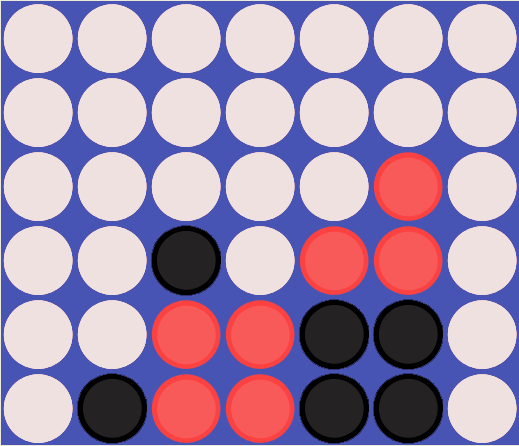
\includegraphics[width=200pt]{img/c4-winning-position.png}
							\caption{Winning position for red player for n=4}						
					\end{center}
				\end{figure}
			